% Options for packages loaded elsewhere
\PassOptionsToPackage{unicode}{hyperref}
\PassOptionsToPackage{hyphens}{url}
\PassOptionsToPackage{dvipsnames,svgnames,x11names}{xcolor}
%
\documentclass[
  11pt,
]{article}
\usepackage{amsmath,amssymb}
\usepackage{iftex}
\ifPDFTeX
  \usepackage[T1]{fontenc}
  \usepackage[utf8]{inputenc}
  \usepackage{textcomp} % provide euro and other symbols
\else % if luatex or xetex
  \usepackage{unicode-math} % this also loads fontspec
  \defaultfontfeatures{Scale=MatchLowercase}
  \defaultfontfeatures[\rmfamily]{Ligatures=TeX,Scale=1}
\fi
\usepackage{lmodern}
\ifPDFTeX\else
  % xetex/luatex font selection
\fi
% Use upquote if available, for straight quotes in verbatim environments
\IfFileExists{upquote.sty}{\usepackage{upquote}}{}
\IfFileExists{microtype.sty}{% use microtype if available
  \usepackage[]{microtype}
  \UseMicrotypeSet[protrusion]{basicmath} % disable protrusion for tt fonts
}{}
\makeatletter
\@ifundefined{KOMAClassName}{% if non-KOMA class
  \IfFileExists{parskip.sty}{%
    \usepackage{parskip}
  }{% else
    \setlength{\parindent}{0pt}
    \setlength{\parskip}{6pt plus 2pt minus 1pt}}
}{% if KOMA class
  \KOMAoptions{parskip=half}}
\makeatother
\usepackage{xcolor}
\usepackage[margin=1in]{geometry}
\usepackage{color}
\usepackage{fancyvrb}
\newcommand{\VerbBar}{|}
\newcommand{\VERB}{\Verb[commandchars=\\\{\}]}
\DefineVerbatimEnvironment{Highlighting}{Verbatim}{commandchars=\\\{\}}
% Add ',fontsize=\small' for more characters per line
\usepackage{framed}
\definecolor{shadecolor}{RGB}{248,248,248}
\newenvironment{Shaded}{\begin{snugshade}}{\end{snugshade}}
\newcommand{\AlertTok}[1]{\textcolor[rgb]{0.94,0.16,0.16}{#1}}
\newcommand{\AnnotationTok}[1]{\textcolor[rgb]{0.56,0.35,0.01}{\textbf{\textit{#1}}}}
\newcommand{\AttributeTok}[1]{\textcolor[rgb]{0.13,0.29,0.53}{#1}}
\newcommand{\BaseNTok}[1]{\textcolor[rgb]{0.00,0.00,0.81}{#1}}
\newcommand{\BuiltInTok}[1]{#1}
\newcommand{\CharTok}[1]{\textcolor[rgb]{0.31,0.60,0.02}{#1}}
\newcommand{\CommentTok}[1]{\textcolor[rgb]{0.56,0.35,0.01}{\textit{#1}}}
\newcommand{\CommentVarTok}[1]{\textcolor[rgb]{0.56,0.35,0.01}{\textbf{\textit{#1}}}}
\newcommand{\ConstantTok}[1]{\textcolor[rgb]{0.56,0.35,0.01}{#1}}
\newcommand{\ControlFlowTok}[1]{\textcolor[rgb]{0.13,0.29,0.53}{\textbf{#1}}}
\newcommand{\DataTypeTok}[1]{\textcolor[rgb]{0.13,0.29,0.53}{#1}}
\newcommand{\DecValTok}[1]{\textcolor[rgb]{0.00,0.00,0.81}{#1}}
\newcommand{\DocumentationTok}[1]{\textcolor[rgb]{0.56,0.35,0.01}{\textbf{\textit{#1}}}}
\newcommand{\ErrorTok}[1]{\textcolor[rgb]{0.64,0.00,0.00}{\textbf{#1}}}
\newcommand{\ExtensionTok}[1]{#1}
\newcommand{\FloatTok}[1]{\textcolor[rgb]{0.00,0.00,0.81}{#1}}
\newcommand{\FunctionTok}[1]{\textcolor[rgb]{0.13,0.29,0.53}{\textbf{#1}}}
\newcommand{\ImportTok}[1]{#1}
\newcommand{\InformationTok}[1]{\textcolor[rgb]{0.56,0.35,0.01}{\textbf{\textit{#1}}}}
\newcommand{\KeywordTok}[1]{\textcolor[rgb]{0.13,0.29,0.53}{\textbf{#1}}}
\newcommand{\NormalTok}[1]{#1}
\newcommand{\OperatorTok}[1]{\textcolor[rgb]{0.81,0.36,0.00}{\textbf{#1}}}
\newcommand{\OtherTok}[1]{\textcolor[rgb]{0.56,0.35,0.01}{#1}}
\newcommand{\PreprocessorTok}[1]{\textcolor[rgb]{0.56,0.35,0.01}{\textit{#1}}}
\newcommand{\RegionMarkerTok}[1]{#1}
\newcommand{\SpecialCharTok}[1]{\textcolor[rgb]{0.81,0.36,0.00}{\textbf{#1}}}
\newcommand{\SpecialStringTok}[1]{\textcolor[rgb]{0.31,0.60,0.02}{#1}}
\newcommand{\StringTok}[1]{\textcolor[rgb]{0.31,0.60,0.02}{#1}}
\newcommand{\VariableTok}[1]{\textcolor[rgb]{0.00,0.00,0.00}{#1}}
\newcommand{\VerbatimStringTok}[1]{\textcolor[rgb]{0.31,0.60,0.02}{#1}}
\newcommand{\WarningTok}[1]{\textcolor[rgb]{0.56,0.35,0.01}{\textbf{\textit{#1}}}}
\usepackage{graphicx}
\makeatletter
\def\maxwidth{\ifdim\Gin@nat@width>\linewidth\linewidth\else\Gin@nat@width\fi}
\def\maxheight{\ifdim\Gin@nat@height>\textheight\textheight\else\Gin@nat@height\fi}
\makeatother
% Scale images if necessary, so that they will not overflow the page
% margins by default, and it is still possible to overwrite the defaults
% using explicit options in \includegraphics[width, height, ...]{}
\setkeys{Gin}{width=\maxwidth,height=\maxheight,keepaspectratio}
% Set default figure placement to htbp
\makeatletter
\def\fps@figure{htbp}
\makeatother
\setlength{\emergencystretch}{3em} % prevent overfull lines
\providecommand{\tightlist}{%
  \setlength{\itemsep}{0pt}\setlength{\parskip}{0pt}}
\setcounter{secnumdepth}{-\maxdimen} % remove section numbering
\usepackage{amsmath,amsfonts,amssymb}
\usepackage{setspace} \doublespacing
\ifLuaTeX
  \usepackage{selnolig}  % disable illegal ligatures
\fi
\usepackage{bookmark}
\IfFileExists{xurl.sty}{\usepackage{xurl}}{} % add URL line breaks if available
\urlstyle{same}
\hypersetup{
  pdftitle={Priors, P-values, and Pfizer: Reanalyzing the BNT162b2 Vaccine Efficacy Trial},
  pdfauthor={Joe Clair, Jay Kumar, and Andrew Tang},
  colorlinks=true,
  linkcolor={Maroon},
  filecolor={Maroon},
  citecolor={Blue},
  urlcolor={blue},
  pdfcreator={LaTeX via pandoc}}

\title{Priors, P-values, and Pfizer: Reanalyzing the BNT162b2 Vaccine
Efficacy Trial}
\author{Joe Clair, Jay Kumar, and Andrew Tang}
\date{March 10, 2026}

\begin{document}
\maketitle

\section{Abstract}\label{abstract}

Write your abstract here.

\section{Keywords}\label{keywords}

\emph{Vaccine Efficacy}, \emph{COVID-19}, \emph{Prior Elicitation},
\emph{Bayesian Analysis}

\newpage

\section{Introduction / Background}\label{introduction-background}

The COVID-19 pandemic, caused by SARS-CoV-2, was one of the most
disruptive global health crises in modern history. The pandemic impacted
global health substantially by not only claiming an estimated 7.1
million lives worldwide (WHO, 2022), but also triggering widespread
economic disruption and social issues, including school closures and
lockdowns across the globe.

In response, Pfizer and BioNTech developed BNT162b2, a two-dose mRNA
vaccine, which was a new approach compared to traditional vaccine
platforms. The vaccine received FDA Emergency Use Authorization in
December 2020 after a large-scale randomized, double-blind,
placebo-controlled Phase 3 trial (Polack et al., 2020). The trial was
designed to run until 170 confirmed COVID-19 cases were observed,
ultimately enrolling 34,922 participants split equally between vaccine
and placebo groups. Vaccine efficacy \(\psi\), defined as the
proportional reduction in infection risk relative to placebo, must
exceed 30\% to meet FDA minimum approval standards. The results are
summarized in Table 1 below.

\begin{center}
    \begin{tabular}{|c|c|c|}
        \hline
        Group & Cases & Sample Size \\
        \hline
        BNT162b2 & 2 & 17411 \\
        \hline
        Placebo & 168 & 17511 \\
        \hline
        Total & 170 & 34922 \\
        \hline
    \end{tabular}
\end{center}

To evaluate vaccine efficacy, each company who developed a vaccine
employed statistical methods to analyze their data. Pfizer used a
Bayesian beta-binomial model and reported 95\% efficacy (Polack et al.,
2020), while another company, Moderna, modeled their data using a
frequentist approach on a similar mRNA vaccine and reported 94.1\%
efficacy (Baden et al., 2021). The fact that two different statistical
frameworks applied to similar mRNA vaccines had similar conclusions was
promising, suggesting the high efficacy of this mRNA holds strong no
matter the statistical framework. However, Pfizer's Bayesian analysis
did not go without scrutiny. Senn (2021) argues that their prior
distribution was reverse-engineered from the FDA's 30\% threshold rather
than reflecting genuine pre-trial belief. We therefore independently
reanalyze the Pfizer trial data using both Bayesian and frequentist
methods, this time using a prior that is more in line with the Bayesian
framework of eliciting our prior beliefs. After our test is done, we
will see if the same conclusions hold. Specifically, we test:

\[H_0: \psi = 0.30 \quad \text{vs} \quad H_1: \psi > 0.30\]

\section{Statistical Methods}\label{statistical-methods}

\subsection{Model}\label{model}

The parameter of interest for this study is,

\[1 - \frac{ \hat \pi_v}{ \hat \pi_p}\] This gives us the efficacy of
the vaccine against Covid-19, where \(\hat \pi_v\) is the probability of
Covid-19 with the vaccine and \(\hat \pi_p\) is the probability of
Covid-19 with the placebo.

Suppose we define the random variable T as the number in the Vaccine
group from the n = 170 Covid-19 cases

The distribution of T can be well approximated by a binomial
distribution which is proved in the appendix

Then,

\[T \sim Binom(n = 170, \pi) \] Where \(\pi\) = P(vaccine \textbar{}
Covid 19 Case) which is equal to,

\[ \pi = \frac{n_1\pi_v}{n_1\pi_v + n_2\pi_p}\] Since
\(n_1 \approx n_2\) so the randomization is 1:1 and so \(\pi\) becomes,
\[\pi  = \frac{\pi_v}{\pi_v + \pi_p}\] Our parameter of interest is the
efficacy which as defined is,
\[ \psi = 1 - \frac{ \pi_v}{  \pi_p} = \frac{\pi_v -\pi_p }{\pi_p}\]
When can represent this in terms of our binomial probability \(\pi\) as,

\[\psi = \frac{1 - 2\pi}{1 - \pi}\] Since the FDA requires at least a
30\% efficacy for the vaccine to be approved our hypothesis that we will
test will be,

\(H_o : \psi = 0.3\) versus \(H_1 : \psi > 0.3\)

\subsection{Likelihood Inference}\label{likelihood-inference}

We will calculate the parameter \(\psi\) using the likelihood estimator
and since \(T \sim Binom(n = 170, \pi)\) the Likelihood function in
terms of \(\pi\) will be,

\[L(\pi) = \binom{n}{k}\pi^k(1-\pi)^{n - k} =\binom{170}{2}\pi^2(1-\pi)^{168} \]
We have,

\[\psi = \frac{1 - 2\pi}{1 - \pi}\] \[(1 - \pi)\psi = 1 - 2\pi\]
\[2\pi- \pi\psi = 1 - \psi\] \[\pi(2 - \psi) = 1 - \psi\]
\[\pi = \frac{1 - \psi}{2 - \psi}\] Since MLEs are invariant to
transformation,

\[L^*(\psi)  =\binom{170}{2}(\frac{1 - \psi}{2 - \psi})^2(1-\frac{1 - \psi}{2 - \psi})^{168} \]
\[l^*(\psi)  =log(\binom{170}{2}) + 2log(1 - \psi) - 2log(2 - \psi) +168log(1-\frac{1 - \psi}{2 - \psi}) \]
\[ =log(\binom{170}{2}) + 2log(1 - \psi) - 2log(2 - \psi) +168log(\frac{1 }{2 - \psi}) \]
\[ =log(\binom{170}{2}) + 2log(1 - \psi) - 2log(2 - \psi) +168log(1) - 168log(2 - \psi) \]
\[l^{*'}(\psi)  = -\frac{2}{1 - \psi} + \frac{170}{2 - \psi} \]
\[-\frac{2}{1 - \psi} + \frac{170}{2 - \psi} = 0\]
\[\frac{170}{2 - \psi} = \frac{2}{1 - \psi}\]
\[170 - 170\psi = 4 - 2\psi\] \[166 = 168\psi\]
\[\hat \psi^{mle} = \frac{166}{168} = 0.98809\]

We will now calculate the confidence interval for our estimate,

We can use the theorem that our estimate is normally distributed with
\(\psi_0\) as the mean and the standard error as
\(\frac{1}{\sqrt{I(\psi_0)}}\), where \(I(\psi_0)\) is the expected
fisher information. To show that n is large enough and that regularity
condition holds for this theorem to be used we need to verify that the
log-likelihood function can be well approximated by a second order
Taylor series around the MLE.

\begin{Shaded}
\begin{Highlighting}[]
\NormalTok{loglik.psi }\OtherTok{\textless{}{-}} \ControlFlowTok{function}\NormalTok{(psi, v, n) \{}
  \FunctionTok{ifelse}\NormalTok{((psi }\SpecialCharTok{\textgreater{}=} \DecValTok{1}\NormalTok{), }\ConstantTok{NA}\NormalTok{,}
\NormalTok{    v }\SpecialCharTok{*} \FunctionTok{log}\NormalTok{(}\DecValTok{1} \SpecialCharTok{{-}}\NormalTok{ psi) }\SpecialCharTok{{-}}\NormalTok{ n }\SpecialCharTok{*} \FunctionTok{log}\NormalTok{(}\DecValTok{2} \SpecialCharTok{{-}}\NormalTok{ psi)}
\NormalTok{  )}
\NormalTok{\}}

\NormalTok{ml.psi }\OtherTok{\textless{}{-}} \FunctionTok{maxLik2}\NormalTok{(}\AttributeTok{loglik =}\NormalTok{ loglik.psi,}
                  \AttributeTok{start =} \FloatTok{0.5}\NormalTok{,}
                  \AttributeTok{v =} \DecValTok{2}\NormalTok{,}
                  \AttributeTok{n =} \DecValTok{170}\NormalTok{)}

\FunctionTok{plot}\NormalTok{(ml.psi, }\AttributeTok{xlim =} \FunctionTok{c}\NormalTok{(}\FloatTok{0.90}\NormalTok{, }\FloatTok{1.00}\NormalTok{)) }\SpecialCharTok{+}
  \FunctionTok{labs}\NormalTok{(}\AttributeTok{title =} \StringTok{"Second order approximation"}\NormalTok{,}
       \AttributeTok{subtitle =} \StringTok{"n = 170, t = 2"}\NormalTok{,}
       \AttributeTok{x =} \FunctionTok{expression}\NormalTok{(psi),}
       \AttributeTok{y =} \StringTok{"Log{-}Likelihood"}\NormalTok{)}
\end{Highlighting}
\end{Shaded}

\begin{verbatim}
## Warning: Using `size` aesthetic for lines was deprecated in ggplot2 3.4.0.
## i Please use `linewidth` instead.
## i The deprecated feature was likely used in the fastR2 package.
##   Please report the issue at <https://github.com/rpruim/fastR2/issues>.
## This warning is displayed once every 8 hours.
## Call `lifecycle::last_lifecycle_warnings()` to see where this warning was
## generated.
\end{verbatim}

\begin{verbatim}
## Warning: Removed 27 rows containing missing values or values outside the scale range
## (`geom_function()`).
\end{verbatim}

\begin{verbatim}
## Warning: Removed 101 rows containing missing values or values outside the scale range
## (`geom_function()`).
\end{verbatim}

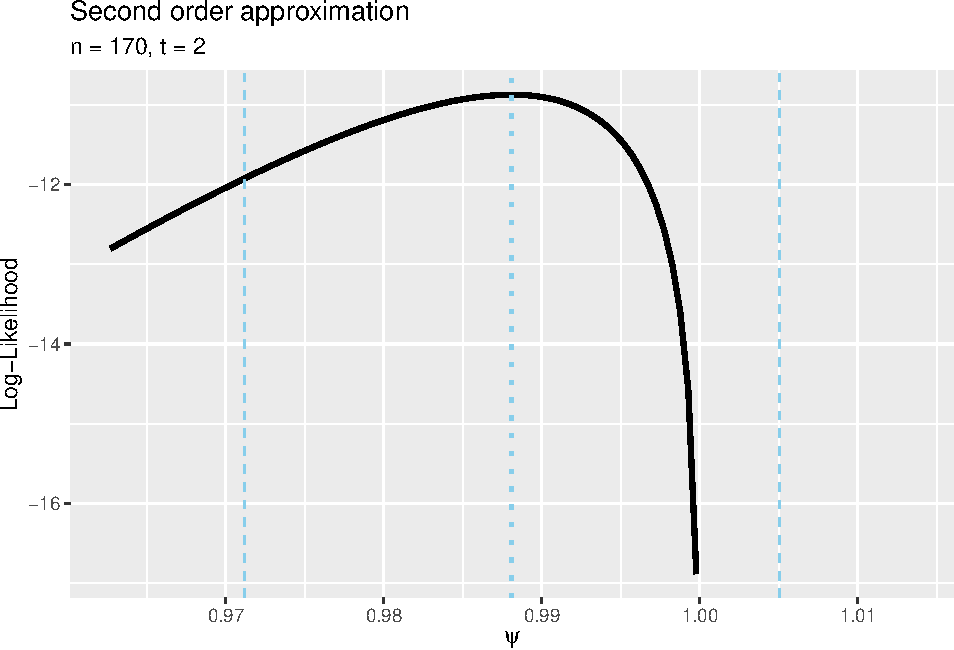
\includegraphics{342-Final-Project_files/figure-latex/unnamed-chunk-1-1.pdf}

We will now calculate the inteval using this distribution of our
estimate, The fisher expected fisher information is given by,

\[I(\psi_0) = E[-\frac{d^2}{d\psi^2}l^*(\psi)]_{\psi = \psi_0}\]
\[-\frac{d^2}{d\psi^2}l^*(\psi) = \frac{2}{1 - \psi} + \frac{170}{(2 - \psi)^2}\]
\[E[-\frac{d^2}{d\psi^2}l^*(\psi)]_{\psi = \psi_0} = \frac{2}{1 - \psi} + \frac{170}{(2 - \psi)^2}\]
\[ = \frac{2}{1 - \frac{166}{168}} + \frac{170}{(2 - \frac{166}{168})^2}\]
\[ = \frac{28392}{85}\] We can calculate a 95\% confidence interval
with,
\[\hat \psi^{mle} \pm z_{\alpha/2}\sqrt{\frac{1}{I(\hat \psi^{mle})}}\]

\begin{Shaded}
\begin{Highlighting}[]
\NormalTok{n }\OtherTok{\textless{}{-}} \DecValTok{170}
\NormalTok{v }\OtherTok{\textless{}{-}} \DecValTok{2}
\NormalTok{psi\_hat }\OtherTok{\textless{}{-}}\NormalTok{ (n }\SpecialCharTok{{-}} \DecValTok{2}\SpecialCharTok{*}\NormalTok{v) }\SpecialCharTok{/}\NormalTok{ (n }\SpecialCharTok{{-}}\NormalTok{ v)}

\NormalTok{I }\OtherTok{\textless{}{-}} \DecValTok{2}\SpecialCharTok{/}\NormalTok{(}\DecValTok{1} \SpecialCharTok{{-}}\NormalTok{ psi\_hat)}\SpecialCharTok{\^{}}\DecValTok{2} \SpecialCharTok{+} \DecValTok{170}\SpecialCharTok{/}\NormalTok{(}\DecValTok{2} \SpecialCharTok{{-}}\NormalTok{ psi\_hat)}\SpecialCharTok{\^{}}\DecValTok{2}

\NormalTok{SE }\OtherTok{\textless{}{-}} \DecValTok{1}\SpecialCharTok{/}\FunctionTok{sqrt}\NormalTok{(I)}

\NormalTok{lower }\OtherTok{\textless{}{-}}\NormalTok{ psi\_hat }\SpecialCharTok{{-}} \FloatTok{1.96} \SpecialCharTok{*}\NormalTok{ SE}
\NormalTok{upper }\OtherTok{\textless{}{-}}\NormalTok{ psi\_hat }\SpecialCharTok{+} \FloatTok{1.96} \SpecialCharTok{*}\NormalTok{ SE}
\FunctionTok{c}\NormalTok{(lower,upper)}
\end{Highlighting}
\end{Shaded}

\begin{verbatim}
## [1] 0.9716923 1.0044982
\end{verbatim}

So our 95\% confidence interval for our estimate will be, (0.9716923,
1.0044982)

We will now calculate the interval through a parametric bootstrap
percentile interval.

To do this we will follow the steps of first repeatedly creating new
samples from the distribution,

\[T \sim Binom(n = 170,  \hat \pi)\] We re-sample from the binomial
distribution using our estimated \(\pi\) from the original sample of the
trials. Then with each sample we will calculate our estimate \(\psi\)
and then for the 95\% confidence interval will take the 2.5th and 97.5th
percentile to create our confidence interval.

\begin{Shaded}
\begin{Highlighting}[]
\FunctionTok{set.seed}\NormalTok{(}\DecValTok{342}\NormalTok{)}

\NormalTok{n }\OtherTok{\textless{}{-}} \DecValTok{170}
\NormalTok{v }\OtherTok{\textless{}{-}} \DecValTok{2}
\NormalTok{pi\_hat }\OtherTok{\textless{}{-}}\NormalTok{ v}\SpecialCharTok{/}\NormalTok{n}
\NormalTok{psi\_hat }\OtherTok{\textless{}{-}}\NormalTok{ (n }\SpecialCharTok{{-}} \DecValTok{2}\SpecialCharTok{*}\NormalTok{v)}\SpecialCharTok{/}\NormalTok{(n }\SpecialCharTok{{-}}\NormalTok{ v)}

\NormalTok{B }\OtherTok{\textless{}{-}} \DecValTok{10000}

\NormalTok{t }\OtherTok{\textless{}{-}} \FunctionTok{rbinom}\NormalTok{(}\AttributeTok{n =}\NormalTok{ B, }\AttributeTok{size =}\NormalTok{ n, }\AttributeTok{prob =}\NormalTok{ pi\_hat)}

\NormalTok{psi }\OtherTok{\textless{}{-}}\NormalTok{ (n }\SpecialCharTok{{-}} \DecValTok{2}\SpecialCharTok{*}\NormalTok{t) }\SpecialCharTok{/}\NormalTok{ (n }\SpecialCharTok{{-}}\NormalTok{ t)}

\FunctionTok{c}\NormalTok{(}\AttributeTok{lower =} \FunctionTok{quantile}\NormalTok{(psi, }\FloatTok{0.025}\NormalTok{),}\AttributeTok{upper =} \FunctionTok{quantile}\NormalTok{(psi, }\FloatTok{0.975}\NormalTok{))}
\end{Highlighting}
\end{Shaded}

\begin{verbatim}
##  lower.2.5% upper.97.5% 
##    0.969697    1.000000
\end{verbatim}

So our 95\% bootstrapped confidence interval will be, (0.969697, 1)

To assess whether the data provide sufficient evidence against \(H_0\),
we use the likelihood ratio test statistic,

\[W = 2[\ell^*(\hat{\psi}^{mle}) - \ell^*(\psi_0)]\] which measures how
much more likely the observed data are under the MLE compared to the
null value \(\psi_0 = 0.3\). Large values of \(W\) indicate the null
hypothesis is not likely given the data. Under \(H_0\), \(W\) follows an
approximate \(\chi^2_1\) distribution for large \(n\), which we use to
compute a P-value. We also compute an empirical P-value by simulating
the distribution of \(W\) under \(H_0\) directly.

\subsection{Bayesian Inference}\label{bayesian-inference}

Before seeing the data, we set two prior beliefs about vaccine efficacy
\(\psi\). We chose \(P(\psi \geq 0.3) = 0.10\) because mRNA vaccines had
never been approved before, and most Phase 3 vaccine trials fail, so we
were skeptical the vaccine would clear the FDA's 30\% bar. We chose
\(P(\psi \geq 0) = 0.60\) given promising immune responses observed in
Phase 1/2 trials (Polack et al., 2020). Following Senn (2021), who
argues Pfizer's prior was reverse-engineered from the FDA threshold
rather than reflecting real prior beliefs, we created our beliefs
directly rather than working backwards from the approval standard. We
now will use the \texttt{beta.select} function in R in order to generate
a beta distribution from our new prior beliefs.

Under our prior beliefs, \begin{align*}
P (\psi \geq 0.3) = 0.1, \ \ \ P (\psi \geq 0) = 0.6.
\end{align*}

When \(\psi = 0.3\), \begin{align*}
\pi = \frac{1-0.3}{2-0.3} = \frac{0.7}{1.7} = \frac{7}{17}.
\end{align*} Thus, \begin{align*}
P(\psi \geq 0.3) = 0.1
\quad \Longleftrightarrow \quad
P\left(\pi \leq \frac{7}{17}\right) = 0.1.
\end{align*}

When \(\psi = 0\), \begin{align*}
\pi = \frac{1-0}{2-0} = \frac{1}{2}.
\end{align*} Thus, \begin{align*}
P(\psi \geq 0) = 0.6
\quad \Longleftrightarrow \quad
P\left(\pi \leq \frac{1}{2}\right) = 0.6.
\end{align*}

So, our conditions for \(\pi\) are \begin{align*}
P\left(\pi \leq \frac{7}{17}\right) = 0.1,
\qquad
P\left(\pi \leq \frac{1}{2}\right) = 0.6.
\end{align*}

Using this to create a beta distribution gives \(Beta (36.40, 38.58)\)
as the prior.

\begin{Shaded}
\begin{Highlighting}[]
\FunctionTok{library}\NormalTok{(LearnBayes)}
\end{Highlighting}
\end{Shaded}

\begin{verbatim}
## Warning: package 'LearnBayes' was built under R version 4.4.3
\end{verbatim}

\begin{Shaded}
\begin{Highlighting}[]
\FunctionTok{beta.select}\NormalTok{(}
  \AttributeTok{quantile1 =} \FunctionTok{list}\NormalTok{(}\AttributeTok{p =} \FloatTok{0.10}\NormalTok{, }\AttributeTok{x =} \DecValTok{7}\SpecialCharTok{/}\DecValTok{17}\NormalTok{),}
  \AttributeTok{quantile2 =} \FunctionTok{list}\NormalTok{(}\AttributeTok{p =} \FloatTok{0.60}\NormalTok{, }\AttributeTok{x =} \FloatTok{0.50}\NormalTok{)}
\NormalTok{)}
\end{Highlighting}
\end{Shaded}

\begin{verbatim}
## [1] 36.40 38.58
\end{verbatim}

Because the Beta distribution is conjugate to the Binomial, the
posterior distribution of \(\pi\) is also a Beta distribution. \[
T \mid \pi \sim \text{Binomial}(n,\pi)
\] and \[
\pi \sim \text{Beta}(a,b),
\] then the posterior distribution is \[
\pi \mid T=t \sim \text{Beta}(a+t,\; b+n-t).
\] For our data, \(n=170\) and \(t=8\), so the posterior distribution is
\[
\pi \mid T=8 \sim \text{Beta}(a+8,\; b+162).
\]

\section{Results}\label{results}

\#hypothesis test findings

Both hypothesis tests provided overwhelming evidence against
\(H_0: \psi = 0.30\). The likelihood ratio test statistic was
\(W = 121.6012\), which under the \(\chi^2_1\) approximation yields a
P-value essentially equal to zero. The empirical P-value, obtained by
simulating 10,000 samples from the null distribution of
\(T \sim Binom(170, \pi_0)\) where \(\pi_0 = 7/17\), was similarly
\(p_{emp} = 0\). Both results provide evidence that the true vaccine
efficacy exceeds the FDA minimum threshold of 30\%

\section{Discussion / Conclusion}\label{discussion-conclusion}

Discuss / conclude here.

\#\#Comment in here about Senn (2021), and how despite criticizing that
the prior was reverse engineered around the 30\% FDA Threshold, the data
was so strong that we still get the same values.

\section{Bibliography}\label{bibliography}

Baden, L. R., El Sahly, H. M., Essink, B., Kotloff, K., Frey, S., Novak,
R., \ldots{} \& Zaks, T. (2021). Efficacy and safety of the mRNA-1273
SARS-CoV-2 vaccine. \emph{New England Journal of Medicine}, 384(5),
403--416.

Polack, F. P., Thomas, S. J., Kitchin, N., Absalon, J., Gurtman, A.,
Lockhart, S., \ldots{} \& Jansen, K. U. (2020). Safety and efficacy of
the BNT162b2 mRNA Covid-19 vaccine. \emph{New England Journal of
Medicine}, 383(27), 2603--2615.

Senn, S. (2021). \emph{Beta testing: The Pfizer/BioNTech statistical
analysis of their Covid-19 vaccine trial}. Error Statistics Philosophy.
Retrieved from
\url{https://errorstatistics.com/2021/01/17/s-senn-beta-testing-the-pfizer-biontech-statistical-analysis-of-their-covid-19-vaccine-trial-guest-post/}

World Health Organization. (2022). \emph{COVID-19 dashboard}. Retrieved
from \url{https://data.who.int/dashboards/covid19/deaths?n=c}

\section{Appendix}\label{appendix}

\subsection{Code}\label{code}

\begin{Shaded}
\begin{Highlighting}[]
\CommentTok{\# You can reference your code in the appendix (sample here).}
\end{Highlighting}
\end{Shaded}

\begin{Shaded}
\begin{Highlighting}[]
\CommentTok{\#Calculating W and then Chi Sq approximation P{-}value}
\NormalTok{n }\OtherTok{\textless{}{-}} \DecValTok{170}
\NormalTok{t }\OtherTok{\textless{}{-}} \DecValTok{8}
\NormalTok{psi\_hat }\OtherTok{\textless{}{-}}\NormalTok{ (n }\SpecialCharTok{{-}} \DecValTok{2}\SpecialCharTok{*}\NormalTok{t) }\SpecialCharTok{/}\NormalTok{ (n }\SpecialCharTok{{-}}\NormalTok{ t)}
\NormalTok{psi\_0 }\OtherTok{\textless{}{-}} \FloatTok{0.3}

\NormalTok{loglik.psi }\OtherTok{\textless{}{-}} \ControlFlowTok{function}\NormalTok{(psi, t, n) \{}
\NormalTok{  t }\SpecialCharTok{*} \FunctionTok{log}\NormalTok{(}\DecValTok{1} \SpecialCharTok{{-}}\NormalTok{ psi) }\SpecialCharTok{{-}}\NormalTok{ n }\SpecialCharTok{*} \FunctionTok{log}\NormalTok{(}\DecValTok{2} \SpecialCharTok{{-}}\NormalTok{ psi)}
\NormalTok{\}}

\NormalTok{W\_obs }\OtherTok{\textless{}{-}} \DecValTok{2} \SpecialCharTok{*}\NormalTok{ (}\FunctionTok{loglik.psi}\NormalTok{(psi\_hat, t, n) }\SpecialCharTok{{-}} \FunctionTok{loglik.psi}\NormalTok{(psi\_0, t, n))}
\NormalTok{W\_obs}
\end{Highlighting}
\end{Shaded}

\begin{verbatim}
## [1] 121.6012
\end{verbatim}

\begin{Shaded}
\begin{Highlighting}[]
\DecValTok{1} \SpecialCharTok{{-}} \FunctionTok{pchisq}\NormalTok{(W\_obs, }\AttributeTok{df =} \DecValTok{1}\NormalTok{)}
\end{Highlighting}
\end{Shaded}

\begin{verbatim}
## [1] 0
\end{verbatim}

\begin{Shaded}
\begin{Highlighting}[]
\CommentTok{\#Empirical P{-}value calcuation}
\FunctionTok{set.seed}\NormalTok{(}\DecValTok{342}\NormalTok{)}
\NormalTok{B }\OtherTok{\textless{}{-}} \DecValTok{10000}
\NormalTok{n }\OtherTok{\textless{}{-}} \DecValTok{170}
\NormalTok{psi\_0 }\OtherTok{\textless{}{-}} \FloatTok{0.3}
\NormalTok{pi\_0 }\OtherTok{\textless{}{-}}\NormalTok{ (}\DecValTok{1} \SpecialCharTok{{-}}\NormalTok{ psi\_0) }\SpecialCharTok{/}\NormalTok{ (}\DecValTok{2} \SpecialCharTok{{-}}\NormalTok{ psi\_0)  }\CommentTok{\# null value of pi}

\NormalTok{w\_star }\OtherTok{\textless{}{-}} \FunctionTok{replicate}\NormalTok{(B, \{}
\NormalTok{  t\_star }\OtherTok{\textless{}{-}} \FunctionTok{rbinom}\NormalTok{(}\DecValTok{1}\NormalTok{, }\AttributeTok{size =}\NormalTok{ n, }\AttributeTok{prob =}\NormalTok{ pi\_0)}
\NormalTok{  psi\_hat\_star }\OtherTok{\textless{}{-}}\NormalTok{ (n }\SpecialCharTok{{-}} \DecValTok{2}\SpecialCharTok{*}\NormalTok{t\_star) }\SpecialCharTok{/}\NormalTok{ (n }\SpecialCharTok{{-}}\NormalTok{ t\_star)}
  \DecValTok{2} \SpecialCharTok{*}\NormalTok{ (}\FunctionTok{loglik.psi}\NormalTok{(psi\_hat\_star, t\_star, n) }\SpecialCharTok{{-}} \FunctionTok{loglik.psi}\NormalTok{(psi\_0, t\_star, n))}
\NormalTok{\})}

\NormalTok{p\_emp }\OtherTok{\textless{}{-}} \FunctionTok{mean}\NormalTok{(w\_star }\SpecialCharTok{\textgreater{}=}\NormalTok{ W\_obs)}
\NormalTok{p\_emp}
\end{Highlighting}
\end{Shaded}

\begin{verbatim}
## [1] 0
\end{verbatim}

\begin{Shaded}
\begin{Highlighting}[]
\NormalTok{df }\OtherTok{\textless{}{-}} \FunctionTok{data.frame}\NormalTok{(}\AttributeTok{w\_star =}\NormalTok{ w\_star)}
\FunctionTok{ggplot}\NormalTok{(df, }\FunctionTok{aes}\NormalTok{(}\AttributeTok{x =}\NormalTok{ w\_star)) }\SpecialCharTok{+}
  \FunctionTok{geom\_histogram}\NormalTok{() }\SpecialCharTok{+}
  \FunctionTok{geom\_vline}\NormalTok{(}\AttributeTok{xintercept =}\NormalTok{ W\_obs) }\SpecialCharTok{+}
  \FunctionTok{labs}\NormalTok{(}
    \AttributeTok{title =} \StringTok{"Empirical Null Distribution of W*"}\NormalTok{,}
    \AttributeTok{x =} \StringTok{"W*"}\NormalTok{,}
    \AttributeTok{y =} \StringTok{"Frequency"}
\NormalTok{  )}
\end{Highlighting}
\end{Shaded}

\begin{verbatim}
## `stat_bin()` using `bins = 30`. Pick better value `binwidth`.
\end{verbatim}

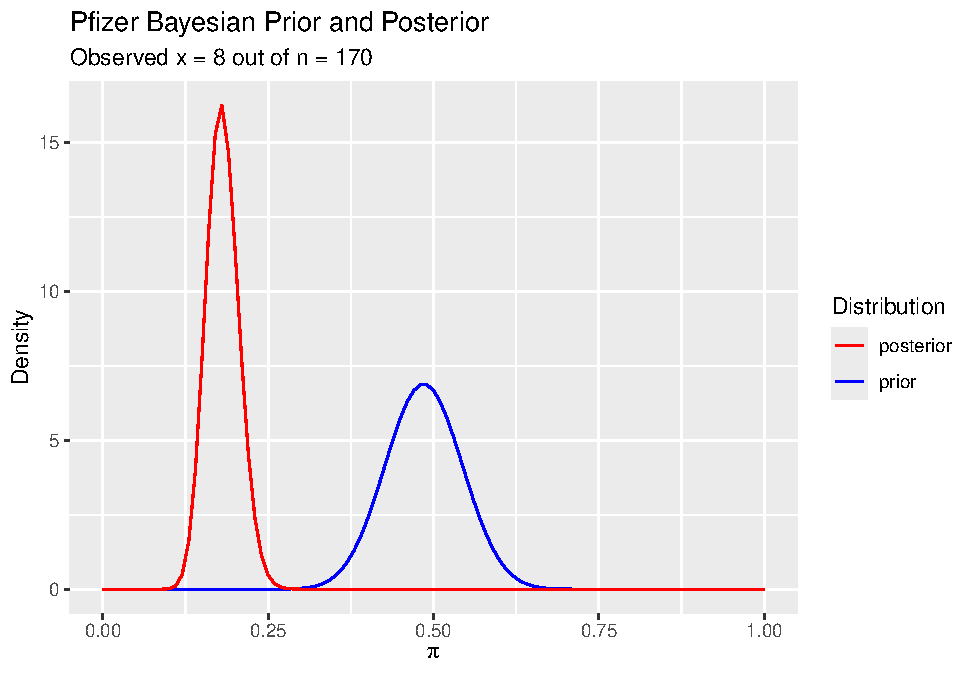
\includegraphics{342-Final-Project_files/figure-latex/unnamed-chunk-7-1.pdf}
\#\# Proofs If applicable, include detailed mathematical derivations or
additional theoretical explanations.

\end{document}
